 \documentclass{article}
 \usepackage{graphicx}
 \graphicspath{ {./images/} }
 
 \begin{document}
 
 \begin{center}
     \Huge\textbf{Homework 1: Sukrit Ganesh}\par
 \end{center}
 
  \noindent\makebox[\linewidth]{\rule{\paperwidth}{0.4pt}}\newline
 
 \begin{center}
      \Large\textbf{Problem 1:} A teacher gives 5 students a multiple choice test, in which each problem is worth 1 point. The median and mean scores turn out to be 9 and 10 points, respectively.\par
 \end{center}
 
 \textbf{Part A: | What is the minimum possible top score?}\newline\newline
 The sum of all scores must be 50, since there are 5 scores with an average of 10. The middle score must be 9 by definition of the median. In order to minimize the top two scores, the bottom two scores must be maximized. Because the median is 9, the bottom two scores can be at most 9. Therefore, the top two scores are 11 and 12 so that the sum of the scores is 50, making 12 the highest score in the set. Although 11.5 is theoretically the lowest max score, all scores must be integers, so 11 and 12 must be used.\newline
 
 Final Answer: 12.\newline
 
 \textbf{Part B: | What is the maximum possible top score?}\newline\newline
 In order to maximize the top score, all other scores must be minimized. The bottom two scores can be 0, while the median score remains 9. The fourth score can be at least 9, because it cannot be less than the median. Hence, the top score is 32, since the sum of the scores must equal 50 (0 + 0 + 9 + 9 + 32).\newline
 
 Final Answer: 32. \newline
 
 \textbf{Part C: | What is the minimum possible standard deviation?}\newline\newline
Standard deviation is a numerical representation of the spread of the data, calculated using the following formula: $\sigma = \sqrt{\frac{1}{N}*\sum_{i=0}^{n}((x_{i}-mean(x_{i})))^2}
$. When the sum of the squared distances from the mean of all the values is minimized, the standard deviation is minimized. In Part A, where we calculated the minimum possible top score, 3 of the data points were equal to 9, while the top two data points were minimized. The range and spread of the data cannot be any smaller. The standard deviation of that set is 1.26.\newline

Final Answer: 1.26.\newline

\textbf{Part D: | What is the maximum possible standard deviation?}\newline\newline
In order to maximize standard deviation, the spread of the data must be maximized. The data set in part B has the maximum spread, since the bottom two values are both 0, while the highest value is 32 (the maximum possible score). The sum of the squared distances from the mean is maximized, and the standard deviation of that set is 11.71.\newline

Final Answer: 11.71. \newline

\newpage
 
 \noindent\makebox[\linewidth]{\rule{\paperwidth}{0.4pt}}\newline
 
 \begin{center}
      \Large\textbf{Problem 2:} Prove that mean and standard deviation of a standardized data set are 0 and 1, respectively.\par
 \end{center}
 
\textbf{Part 1:} The first step to standardize data is to shift the data left or right by the value of the mean. In other words, we subtract the mean from every single data point.\newline

We must prove that after this shift, the mean is 0.

 \begin{displaymath}
\frac{1}{N} * \sum_{i=1}^{n}(x_{i}-mean({x_{i}})) = 0
\end{displaymath}

Let's use the left hand side.

\begin{equation}
\frac{1}{N} * \sum_{i=1}^{n}(x_{i}-mean({x_{i}}))
\end{equation}
  
\begin{equation}  
\frac{1}{N} * \sum_{i=1}^{n}(x_{i}) - \frac{1}{N} * \sum_{i=1}^{n}mean({x_{i}})
\end{equation}

\begin{equation}  
\frac{1}{N} * \sum_{i=1}^{n}(x_{i}) - \frac{1}{N} * N *mean({x_{i}})
\end{equation}

We can notice that the left side is merely the definition of the mean,
while on the right side, \[\frac{1}{N}*N\] cancels out to become 1.

\begin{equation}  
mean({x_{i}}) - mean({x_{i}}) = 0
\end{equation}

We prove that the mean of the shifted data is 0.\newline

The second step in standardization is to divide every single data point by the standard deviation. \newline

We have to prove that the standard deviation of the standardized data is 1. The following is the formula for standard deviation:

\begin{equation}  
\sigma = \sqrt{\frac{1}{N}*\sum_{i=0}^{n}((x_{i}-mean(x_{i})))^2}
\end{equation}

We will use the right-hand side of the equation. Because we have already shifted the data, the mean is 0.

\begin{equation}  
\sqrt{\frac{1}{N}*\sum_{i=0}^{n}(x_{i})^2}
\end{equation}

When data is standardized, we divide every single data point by the standard deviation. We substitute every $x_{i}$ with  $\frac{x_{i}}{\sigma}$. Hence, we get the following expression:

\begin{equation}  
\sqrt{\frac{1}{N}*\sum_{i=0}^{n}(\frac{x_{i}}{\sigma})^2}
\end{equation}

A simple expansion and rearrangement 

\begin{equation}  
\sqrt{\sum_{i=0}^{n}\frac{1}{N}*x_{i}^2*\frac{1}{\sigma}*\frac{1}{\sigma}}
\end{equation}

We know by definition that the formula for variance (the square of standard deviation) when the mean is 0 is the following:

\begin{equation}  
\sigma^2 = \sum_{i=0}^{n}\frac{1}{N}*{x_{i}}^2.
\end{equation}

Hence, we can use it to simplify the expression and subsequently prove that the standard deviation is 1.

\begin{equation}  
\sqrt{\sigma^2*\frac{1}{\sigma}*\frac{1}{\sigma}} = 1
\end{equation}

Q.E.D :)

\newpage
 
\begin{center}
      \Large\textbf{Problem 3:} You can find a dataset giving the cost (in 1976 US dollars), number of megawatts, and year of construction of a set of nuclear power plants at http://lib.stat.cmu.edu/DASL/Datafiles/NuclearPlants.html.\par
\end{center}

\textbf{Part A: | Are there outliers in this data?}\newline\newline
 Yes, there are indeed outliers. A box and whisker plot of the date feature reveals two points more than 1.5 times the IQR away from the 75th percentile mark.\newline
 
 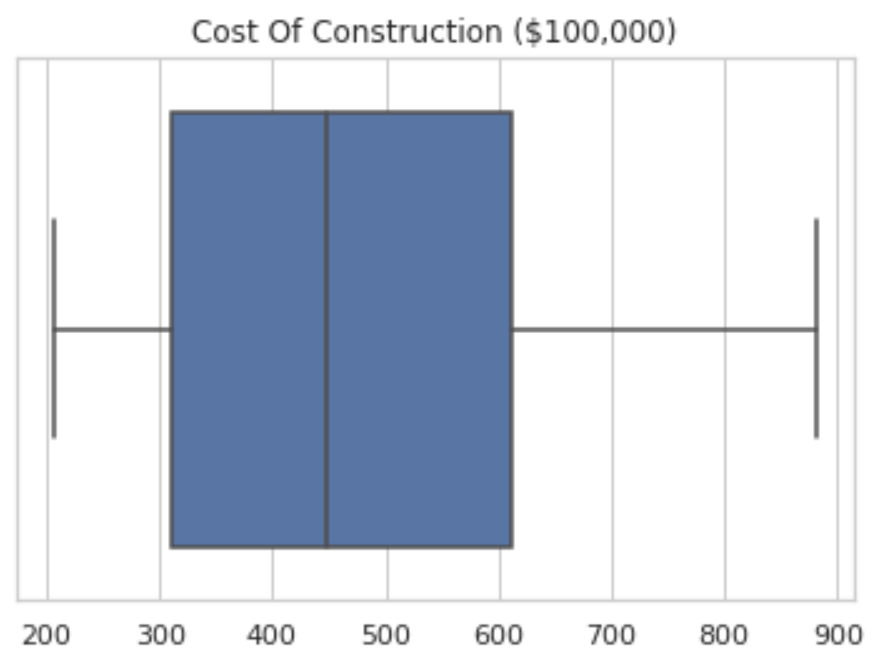
\includegraphics[width=.3\textwidth]{HW1_11.PNG}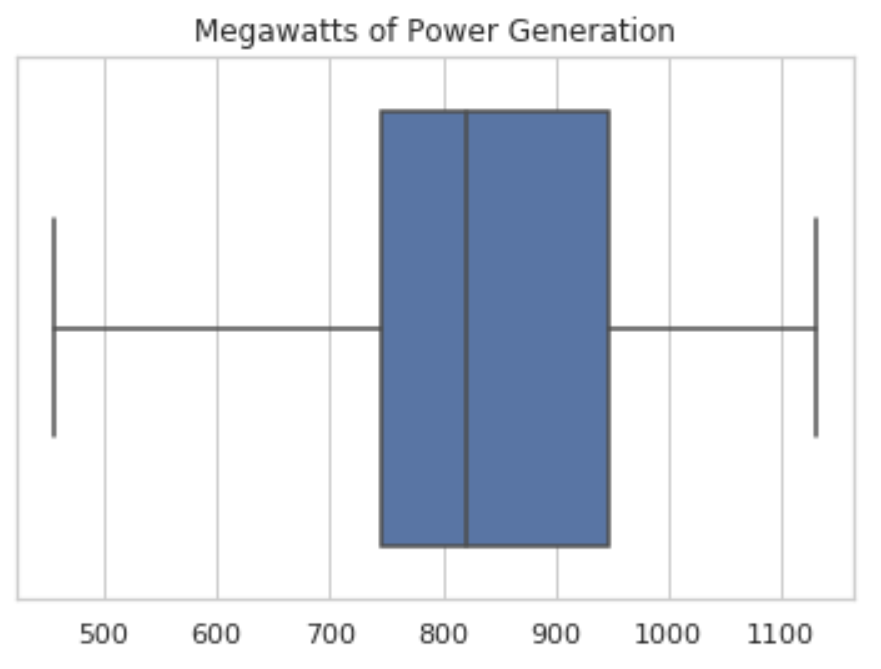
\includegraphics[width=.3\textwidth]{HW1_12.PNG}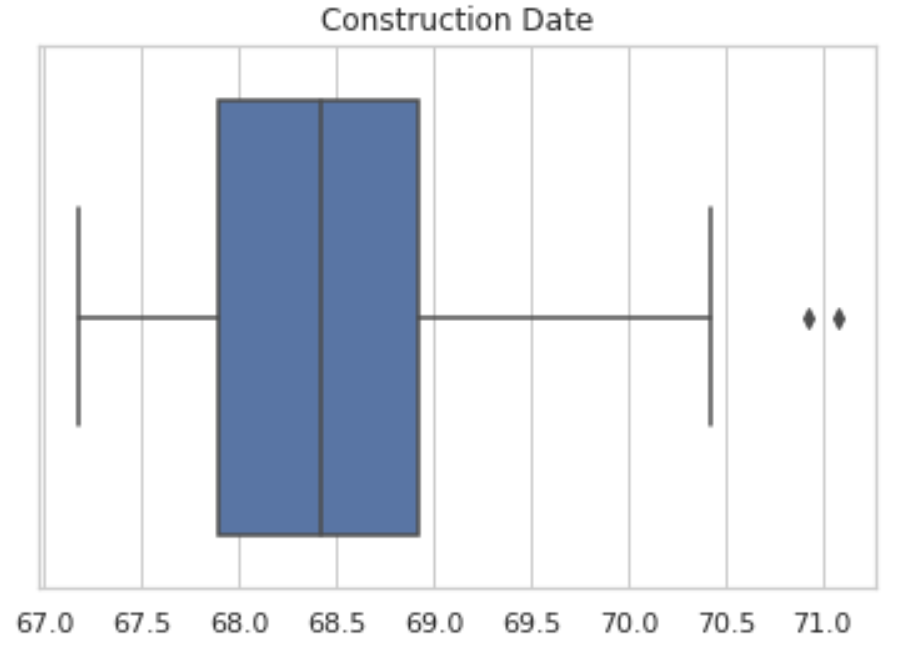
\includegraphics[width=.3\textwidth]{HW1_13.PNG}
 
 Final Answer: Yes: 70.92 and 71.08 are the outliers.\newline
 
 \textbf{Part B: | What is the mean cost of a power plant? What is the standard deviation?}\newline
 
 Final Answer: The mean cost (in terms of \$100,000) and standard deviation are 461.56 and 167.44, respectively (used numpy mean and std functions).\newline
 
 \textbf{Part C: | What is the mean cost per megawatt? What is the standard deviation?}\newline
 
 Final Answer: Yes: The mean cost per megawatt and standard deviation (in terms of \$100,000) are 0.57  and 0.18, respectively (used numpy mean and std functions).\newline
 
 \textbf{Part D: | Plot a histogram of the cost per megawatt. Is it skewed? Why?}\newline\newline
 As seen in the histogram, the data is not skewed. The normal distribution curve produced by seaborn is rouughly symmetrical, and both the mean and median (0.57 and 0.58, respectively) of the data are very close together, indicating only negligible skew. \newline
 
 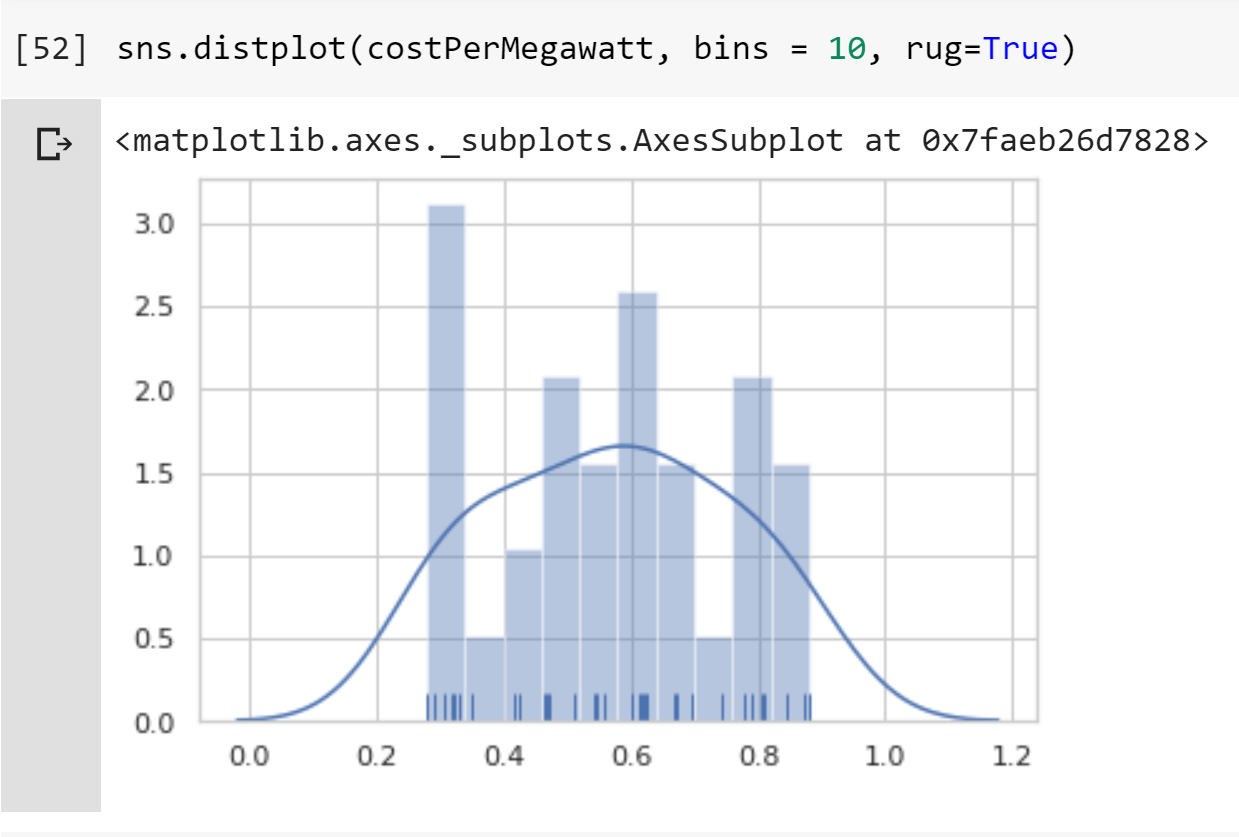
\includegraphics{HW1_2.PNG}
 
 Final Answer: The data is \textbf{not} skewed. \newline
 
 \newpage
 
 \begin{center}
      \Large\textbf{Problem 4:} You can find a dataset giving the sodium content and calorie content of three types of hot dog at http://lib.stat.cmu.edu/DASL/Datafiles/Hotdogs.html. The types are Beef, Poultry, and Meat (a rather disturbingly vague label). Use class-conditional histograms to compare these three types of hot dog with respect to sodium content and calories.\par
 \end{center}

 In the histograms, the red bars represent beef, the pink bars represent meat, and the yellow bars represent poultry. Clearly, beef tends to have lower quantities of sodium as well as fewer calories, while poultry has the highest. In both graphs, the beef histograms are skewed right, while the poultry histograms are skewed left. All three hot dog distributions have similar ranges, but the median of the "meat" hot dogs falls in between the meat and poultry hot dogs. The meat hot dogs have a roughly normal (albeit far from perfect) distribution. It seems as if "meat" is a mix of beef and poultry, since the meat distribution appears to have a mean and median found between the respective means and medians of beef and poultry hot dogs. Since beef is right skewed and poultry is left skewed, it would be logical to conclude that a plot of a composite hot dog made with half poultry and half beef would not be skewed. 
 
 On a side note, beef hot dogs appear to have lower sodium and caloric contents, indicating that either beef hot dogs contain less meat OR beef contains fewer calories and less sodium than poultry. \newline
 
 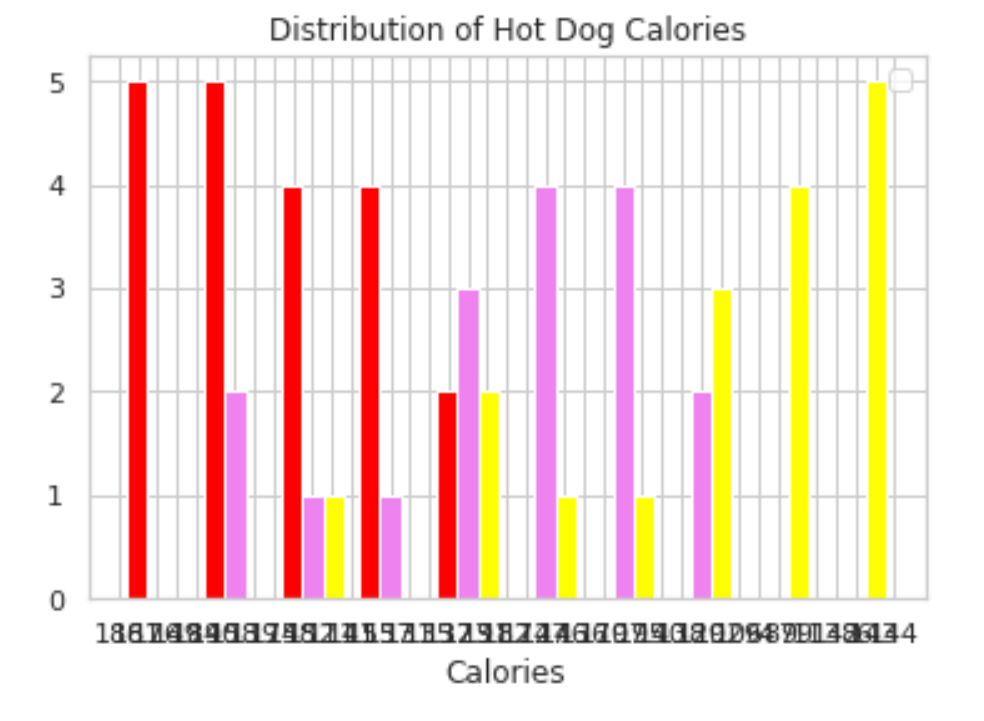
\includegraphics{HW1_3.PNG}
 \newline
 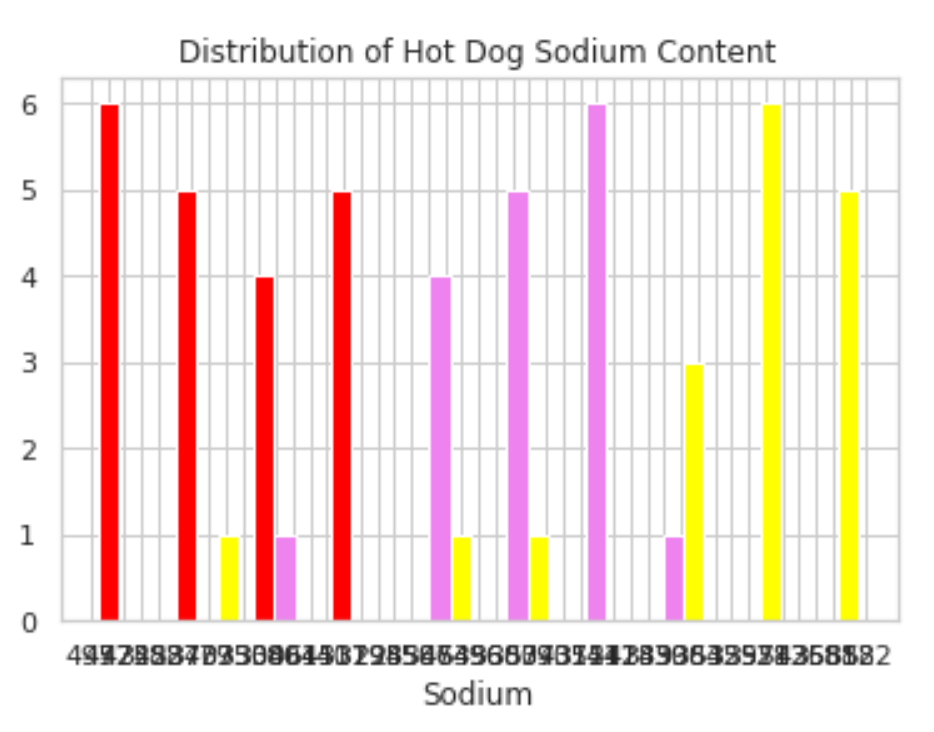
\includegraphics{HW1_4.PNG}
 \newline
 
 \newpage
 
 \begin{center}
      \Large\textbf{Problem 5:}You will find a dataset giving (among other things) the number of 3 or more syllable words in advertising copy appearing in magazines at http://lib.stat.cmu.edu/DASL/Datafiles/magadsdat.html. The magazines are grouped by the education level of their readers; the groups are 1, 2, and 3 (the variable is called GRP in the data).\par
 \end{center}
 
 \textbf{Part A: | Use a box plot to compare the number of three or more syllable  words for the ads in magazines in these three groups. What do you    see?}\newline\newline
 
Group 1 magazines have the highest median frequency of three-syllable words in ads, while Group 2 has the least. The IRQ and range for group 3 is the lowest, suggesting that the majority of magazines have a similar quantity of 3-syllable words in their advertisements. However, group 3 also has the most outliers, suggesting that some magazines may contain specialized ads with a large quantity of 3-syllable words. Group 1 and 3 magazines have the most evenly divided IQR, while Group 2 is heavily skewed right as evidenced by the much larger upper half of the IQR and longer upper whisker. Group 1 also appears to have the largest stanard deviation. Because the whiskers and halves of the IQR are similar in length, however, Group 1 likely has have a uniform distribution rather than a normal distribution. \newline
 
 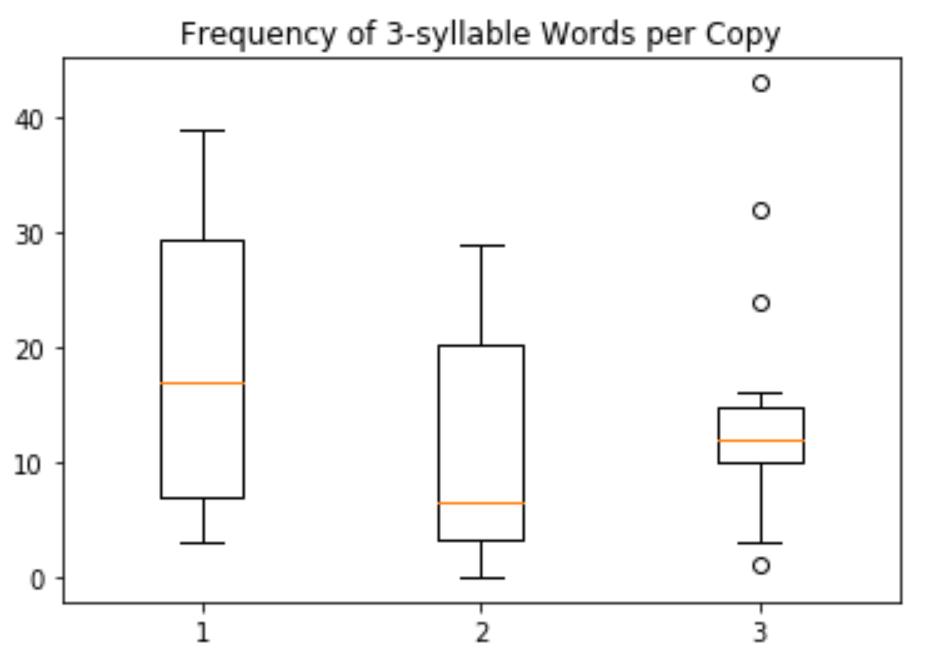
\includegraphics{HW1_5.PNG}
 
 \newline

 \textbf{Part B: | Use a box plot to compare the number of sentences appearing in the ads in magazines in these three groups. What do you see?}\newline\newline
 
All three magazine groups have relatively similar median number of sentences in advertisements, group 2 has a slightly lower median. In group 2, the upper half of the interquartile range is significantly longer than the lower half, indicating a strong right-skew. Furthermore, Group 3 once again has the most outliers, although these outliers are on the lower rather than the upper end. Group 1 has an evenly divided IQR and whiskers roughly equal to the halves of the IQR in length, indicating a uniform distribution. Additionally, group 2 has the largest range, while Group 3 has the smallest range and the smallest standard deviation (excluding outliers). As with the frequency of 3-syllable words, none of the groups have a left-skew.\newline
 
 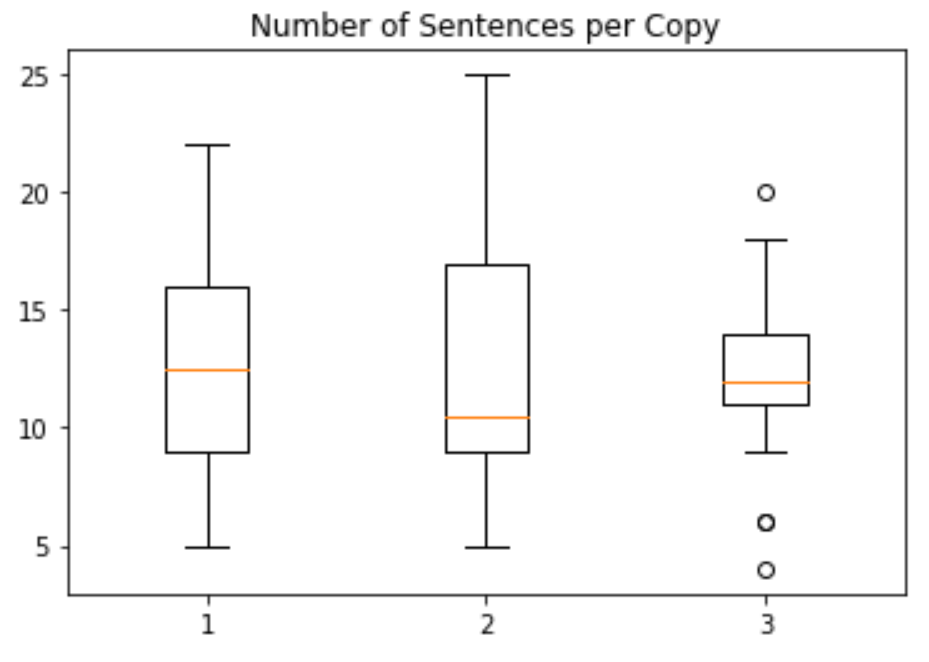
\includegraphics{HW1_6.PNG}
 
 
\end{document}

